\documentclass{scrartcl}
\usepackage[a4paper,left=3cm,right=3cm,top=3cm,bottom=3cm]{geometry}

\usepackage[utf8]{inputenc}
\usepackage[T1]{fontenc}
\usepackage{lmodern}
\usepackage[ngerman]{babel}
\usepackage{amsmath}
\usepackage{caption}
\usepackage{graphicx}
\usepackage{subfig}
\usepackage{hyperref}
\usepackage{listings}
\usepackage{listings}
\usepackage{color}

\definecolor{codegreen}{rgb}{0,0.6,0}
\definecolor{codegray}{rgb}{0.5,0.5,0.5}
\definecolor{codepurple}{rgb}{0.58,0,0.82}
\definecolor{codered}{rgb}{0.8, 0.2, 0.2}
\definecolor{backcolour}{rgb}{0.95,0.95,0.96}

\lstdefinelanguage{JavaScript}{
  keywords={typeof, new, true, false, catch, function, return, null, try, catch, switch, const, var, if, in, while, do, else, case, break},
  keywordstyle=\color{blue}\bfseries,
  ndkeywords={class, export, boolean, throw, implements, import, this},
  ndkeywordstyle=\color{codegray}\bfseries,
  identifierstyle=\color{black},
  sensitive=false,
  comment=[l]{//},
  morecomment=[s]{/*}{*/},
  commentstyle=\color{codepurple}\ttfamily,
  stringstyle=\color{codered}\ttfamily,
  morestring=[b]',
  morestring=[b]"
}
\lstdefinestyle{normal}{
    backgroundcolor=\color{backcolour},   
    commentstyle=\color{codegreen},
    keywordstyle=\color{magenta},
    numberstyle=\tiny\color{codegray},
    stringstyle=\color{codepurple},
    basicstyle=\ttfamily\footnotesize,
    breakatwhitespace=false,         
    breaklines=true,                 
    captionpos=b,                    
    keepspaces=true,                 
    numbers=left,                    
    numbersep=5pt,                  
    showspaces=false,                
    showstringspaces=false,
    showtabs=false,                  
    tabsize=2
}

\lstset{style=normal}

\hypersetup{
    colorlinks,
    citecolor=black,
    filecolor=black,
    linkcolor=black,
    urlcolor=black
}

\begin{document}
%%% Deckblatt
\begin{center}
    \thispagestyle{empty}
    \textbf{Berufsschule für Informationstechnik}

    Am Beruflichen Schulzentrum für Elektrotechnik

    Strehlener Platz 2, 01219 Dresden

    \vfill 
        \LARGE{\textbf{Auswertung und Reflexion}}
        \linebreak
        
        \large{Version 1.0}
        \linebreak
        \linebreak

        \large{IT20/2}
        \linebreak
        \large{Lernfeld 9}
        \linebreak
        \linebreak

        \large{Paul Görtler}
        
        \large{Vincent Jablonski}  

        \large{Marcus Böhme}  
        \linebreak

        \large \today
    \vfill    
\end{center}
\newpage
\setcounter{page}{1}
%%% Deckblatt

\tableofcontents
\newpage

\begin{flushleft}
    \section{Soll-Ist-Vergleich}
    
    \subsection{Projektplanung}
    \textbf{Zielvorstellung:} \newline
    Erfolgreiches erstellen einer übersichtlichen Projektplanung. \newline
    \textbf{Erreichtes Ergebnis:} \newline
    Die erstellte Projektplanung ist übersichtlich und leicht zu verstehen. Die Umsetzung war dementsprechend erfolgreich. \newline

    \subsection{Netzinfrastruktur}
    \textbf{Zielvorstellung:} \newline
    Erfolgreiches erstellen einer durch das Projekt geforderten Netzinfrastruktur. \newline
    \textbf{Erreichtes Ergebnis:} \newline
    Das Erstellen der Netzinfrastruktur war erfolgreich und erfolgte innerhalb kürzester Zeit jedoch lies die Umsetzung keine Komplikationen aus. \newline

    \subsection{Firewall-System}
    \textbf{Zielvorstellung:} \newline
    Erfolgreiches erstellen / konfigurieren des Firewall-Systems. \newline
    \textbf{Erreichtes Ergebnis:} \newline
    Das Erstellen / konfigurieren des Firewall-Systems war erfolgreich. Kleinere Komplikationen blockierten eine schnelle Umsetzung. \newline

    \subsection{DNS und DHCP}
    \textbf{Zielvorstellung:} \newline
    Erfolgreiches konfigurieren von DNS und DHCP. \newline
    \textbf{Erreichtes Ergebnis:} \newline
    Die Konfiguration von DNS und DHCP war problemlos möglich. \newline
 
    \newpage

    \subsection{Web-Server}
    \textbf{Zielvorstellung:} \newline
    Erfolgreiches programmieren eines eigenen Web-Servers sowie das Erstellen und programmieren eines Ticketsystems. \newline
    \textbf{Erreichtes Ergebnis:} \newline
    Die Programmierung des Web-Servers und des Ticketsystems war erfolgreich und verlief ohne Probleme. \newline

    \subsection{Datenbank-Server }
    \textbf{Zielvorstellung:} \newline
    Erfolgreiches erstellen und konfigurieren einer MariaDB Datenbank. Programmieren einer API für den Datenbank-Server. \newline
    \textbf{Erreichtes Ergebnis:} \newline
    Das Erstellen und die Konfiguration der MariaDB Datenbank war erfolgreich. Die Programmierung einer API für den Datenbank-Server war ebenso erfolgreich und verlief ohne Probleme. \newline
 
    \section{Ursachen für Defizite in der Umsetzung}
    Hauptsächlich kam es aufgrund fehlender Erfahrung zu Defiziten in der Umsetzung der einzelnen Projektziele. Ein Gewisser grad an Vorwissen im Umgang mit einzelnen Softwarelösungen wäre zu empfehlen. Im Bereich IPFire fehlte besonders am Anfang eine gewisse Routine im Umgang mit der Software. Krankheitsfälle innerhalb des Projektteams führten ebenso zu Verzögerungen.


    \newpage

    \section{Reflektieren der Arbeitsergebnisse}
    \subsection{Realer Arbeitsaufwand}
    Im folgenden Gantt-Diagramm ist der reale Arbeitsaufwand zu erkennen. Die Farbe Orange kennzeichnet den realen Arbeitsaufwand einer Aufgabe.
    \captionof{figure}{Gantt-Diagramm}
    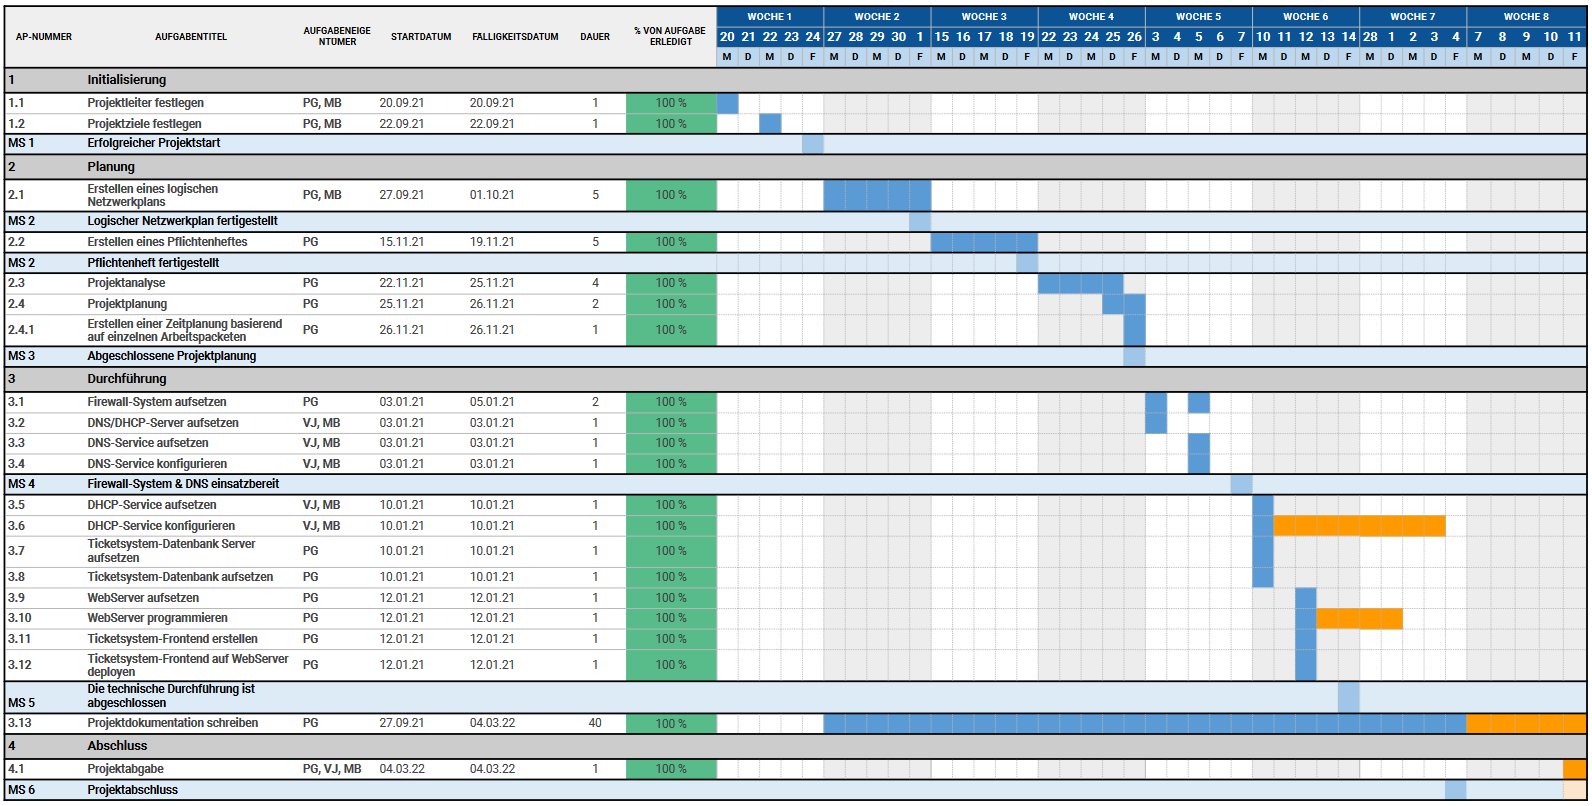
\includegraphics[width=\linewidth]{img/Gantt.PNG}
    \subsection{Abweichungen zwischen Planung und realer Umsetzung}
    Durch eine Verzögerung bei der Konfiguration des DHCP Services und bei der Programmierung des Web-Servers kam es zu einer längeren Bearbeitungszeit der Projektdokumentation(en). Aufgrund von Krankheitsfällen innerhalb des Projektteams kam es ebenso zu Verzögerungen. \newline

    Die Projektabgabe wurde durch Herrn Hempel umdatiert.

    \section{Optimierungsvorschläge zur Projektrealisierung}
    Im Großen und Ganzen ist das Projektteam mit der finalen Projektrealisierung voll und ganz zufrieden. Für das Projektteam lässt sich geschlossen sagen, das mehr Zeit im direkten Arbeiten miteinander große Vorteile mit sich gebracht hätte. \newline
    
    Weiterhin gilt natürlich für jedes Projekt und seine Bestandteile eine gewisse Steigerungsfähigkeit. Auch dieses Projekt ist an einigen stellen durchaus optimierbar.


\end{flushleft}
\end{document}